\documentclass{standalone}
%\url{http://tex.stackexchange.com/q/141259/86}
\usepackage{tikz}
\usetikzlibrary{chains}
\begin{document}
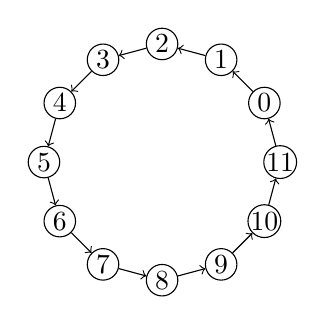
\begin{tikzpicture}[start chain=circle placed {at=(\tikzchaincount*30:1.5)},regular/.style={draw,circle,inner sep=0,minimum size=4mm}]
\foreach \i in {0,...,11}
  \node [on chain, regular] (\i) {\i};
\foreach[evaluate=\i as \ni using {int(mod(\i+1,12))}] \i in {0,...,11}
  \draw [->] (\i) to (\ni);
\end{tikzpicture}
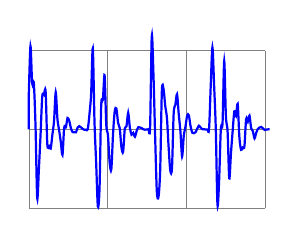
\begin{tikzpicture}[
declare function={
excitation(\t,\w) = sin(\t*\w);
noise = rnd - 0.5;
source(\t) = excitation(\t,20) + noise;
filter(\t) = 1 - abs(sin(mod(\t, 90)));
speech(\t) = 1 + source(\t)*filter(\t);
}
]
\draw [help lines] (0,0) grid (3,2);
\draw [blue, thick, x=0.0085cm, y=1cm] (0,1) --
plot [domain=0:360, samples=144, smooth] (\x,{speech(\x)});
\end{tikzpicture}
\end{document}
